\documentclass[crop=false,10pt]{standalone}
\usepackage{standard}

\begin{document}
  \section{Inference} % (fold)
  \label{sec:Inference}
    The general inference for an RBM can be done by using the Gibbs sampling method explained in the last chapter.
    Here we will explicitly talk about the inference for the collaborative filtering problem.
    Figure \ref{fig:rbm-inference-example} shows such an application in a schematic example.
    \begin{figure*}[h]
      \center
      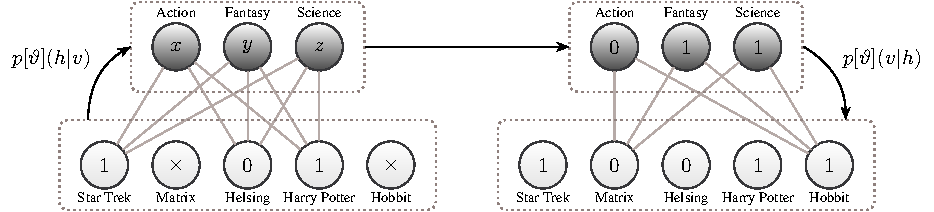
\includegraphics[width=0.9\textwidth]{figures/rbm-inference-example.pdf}
      \caption{%
        The figure shows the application of inference to the prediction of movie ratings for users.
      }
      \label{fig:rbm-inference-example}
    \end{figure*}

    First, we get the vector of rated and unrated movies from a given user.
    We then have to sample the hidden values by using only the values for the rated movies via the a posterior probability.
    After this we are now able to sample values for the unrated movies again by using the a posterior probability.
    The values sampled are then the predictions of the user ratings.
  % section Inference (end)
\end{document}